% -*- coding: iso-8859-1 -*-

\documentclass[blue]{beamer}
\usepackage[latin1]{inputenc}
\usepackage{tikz}
\usetikzlibrary{shapes,arrows}
\pgfdeclarelayer{background}
\pgfdeclarelayer{foreground}
\pgfsetlayers{background,main,foreground}

\usepackage{pgfpages}
%\pgfpagesuselayout{resize to}[a4paper,landscape]
%\pgfpagesuselayout{2 on 1}[a4paper,border shrink=6mm]
%\pgfpagesuselayout{4 on 1}[a4paper,border shrink=5mm,landscape]
%\pgfpagesuselayout{8 on 1}[a4paper,border shrink=3mm]

\mode<presentation>
{
   \usetheme{Singapore}
   \setbeamertemplate{navigation symbols}{}
   \setbeamertemplate{items}[ball]
   \setbeamertemplate{sections/subsections in toc}[ball]
}

\title{Title} 
\subtitle{subtitle} 

\author[shortauthors]{
  Samuel \textsc{Colin}\inst{1} \and 
  Samuel \textsc{Hivernal}\inst{2}
}

\institute[shortinstitutes]{\inst{1}Institute1 
  \and \inst{2}Institute2
  \and Unrelated thing}
\date{\today}

\logo{

\includegraphics[height=0.5cm]{graphics-pdf}
} 

\AtBeginSection[]
{
   \begin{frame}<beamer>
     \frametitle{Outline}
     \tableofcontents%[currentsection,currentsubsection]
   \end{frame}
}

\begin{document}

\begin{frame}
  \titlepage
\end{frame}


\section{Section 1}
\label{sec:section-1}

\begin{frame}
  \frametitle{Title for section \ref{sec:section-1}}
  \framesubtitle{yup, section \ref{sec:section-1}}

\end{frame}

\subsection{Subsection 1-1}
\label{sec:subsection-1-1}

\begin{frame}
  \frametitle{Subsection~\ref{sec:subsection-1-1} ? Wow}
  \framesubtitle{a subsection, right}

Hey, I cite \cite{test06}.

\end{frame}

\subsection{Subsection 1-2}
\label{sec:subsection-1-2}

\begin{frame}
  \frametitle{We're at subsection~\ref{sec:subsection-1-2}}
  \framesubtitle{true, true}

Let me reference something far, such as \ref{sec:subsection-3-3}.

\end{frame}


\section{Section 2}
\label{sec:section-2}

\begin{frame}
  \frametitle{Title for section \ref{sec:section-2}}
  \framesubtitle{no subsection here}

And here I cite \cite{test04}.

\end{frame}

\begin{frame}
  \frametitle{Title for section \ref{sec:section-2} (cont'd)}
  \framesubtitle{Told you there was no subsection}

\end{frame}



\section{Section 3}
\label{sec:section-3}

\begin{frame}
  \frametitle{Title for section \ref{sec:section-3}}
  \framesubtitle{another section...}

\end{frame}


\subsection{Subsection 3-1}
\label{sec:subsection-3-1}

\begin{frame}
  \frametitle{Many frames in a subsection}
  \framesubtitle{subsection \ref{sec:subsection-3-1}, btw}

  \vfill
  \vfill
  \vfill
  \begin{center}
  \begin{tikzpicture}[x=15em,y=8em,overlay]

    \path<2-> (-0.5,-0.5) node (AlarmStatus) {\textsf{AlarmStatus}};
    \path<5-> (0.5,-0.5) node (cardStatus) {$\mathsf{1..card(\mbox{\textsf{AlarmStatus}})}$};
    \path<1-> (-0.5,0.5) node (alarmids) {\textsf{alarms\_ids}};
    \path<3-> (0.5,0.5) node (natids) {\textsf{nat\_ids}};

    \draw<2->[->]   (alarmids) -- node[sloped,below]{\textsf{alarms\_status}} node[sloped,above]{\textbf{(1)}} (AlarmStatus);
    \draw<3->[>->>] (alarmids) -- node[above]{\textsf{id\_cast}} node[below]{\textbf{(2.1)}} (natids);
    \draw<5->[>->>] (AlarmStatus) -- node[below]{\textsf{status\_cast}} node[above]{\textbf{(2.3)}} (cardStatus);
    \draw<5->[->]   (natids) -- node[sloped,above]{\textsf{status\_nn}} node[sloped,below]{\textbf{(2.3)}} (cardStatus);
    \draw<4->[->]   (natids) -- node[sloped,above]{\textsf{nat\_status}} node[sloped,below]{\textbf{(2.2)}} (AlarmStatus);
  \end{tikzpicture}    
  \end{center}

  \vfill
  \vfill
  \vfill
  \vfill

  \begin{overlayarea}{0.99\textwidth}{0.2\textheight}
  \only<1>{The beginning}
  \only<2>{Transform the data structures}
  \only<3>{Cast the simple variables}
  \only<4>{Cast the domains of the functional variables}
  \only<5>{Cast the codomains of the functional variables (and do the
    operations calls after that)}
  \end{overlayarea}


\end{frame}

\begin{frame}
  \frametitle{Again for \ref{sec:subsection-3-1}}
  \framesubtitle{yup...}

\end{frame}

\begin{frame}
  \frametitle{The end for \ref{sec:subsection-3-1}}
  \framesubtitle{but wait for subsection~\ref{sec:subsection-3-2}}

\end{frame}

\subsection{Subsection 3-2}
\label{sec:subsection-3-2}

\begin{frame}
  \frametitle{Only 2 frames in this subsection}
  \framesubtitle{promised}

\end{frame}

\begin{frame}
  \frametitle{see, told ya}
  \framesubtitle{\ref{sec:subsection-3-2}, btw}

\end{frame}

\subsection{Subsection 3-3}
\label{sec:subsection-3-3}

\begin{frame}
  \frametitle{Only one frame here}
  \framesubtitle{\ref{sec:subsection-3-3}}

\end{frame}

\appendix

\section*{References}

\begin{frame}[allowframebreaks]
  \frametitle{References}
    
  \setbeamerfont{bibliography entry author}{size=\scriptsize}

  \bibliographystyle{apalike}
  \bibliography{../../common/bibliography/biblio2}
\end{frame}

\end{document}


%%% Local Variables: 
%%% mode: latex
%%% TeX-master: t
%%% End: 
